\chapter{Implementation}\label{cha:implementation}
\section{System overview}
An overview of the implemented system is shown in Figure \ref{fig:sys_overview}.
\begin{figure}[H]
    \begin{center}
        \begin{tikzpicture}[node distance = 3cm, auto]
            \node[block] (init){Landing area input};
            \node[block, right of=init] (land){Landing sequence calculation};
            \node[block, below of=land] (obst){Obstacle database};
            \node[block, above of=land] (wind){Wind estimation};
            \node[block, right of=land] (mp){Motion planner};
            \node[block, above of=mp] (gps){Positioning system};
            \node[block, right of=mp] (traj){Waypoint controller};

            \path[line] (init) - > node{$\landing$} (land); 
            \path[line] (obst) - > node[midway, right]{$\xobst$} (land);
            \path[line] (obst) - > node[midway, right]{$\xobst$} (mp);
            \path[line] (wind) - > node[midway, right]{$\windvec$} (land);
            \path[line] (wind) - > node[midway, right]{$\windvec$} (mp);
            \path[line] (land) - > node[midway]{$x_g$} (mp);
            \path[line] (gps) - > node[midway, right]{$x_0$} (mp);
            \path[line] (mp) - > node[midway]{$\mathcal{M}$} (traj);
        \end{tikzpicture}
    \end{center}
    \caption{System overview}
    \label{fig:sys_overview}
\end{figure}
The \ac{uav} is assumed to be equipped with a wind estimation system which can measure the current wind vector $\windvec$, and a positioning system which estimates the current position of the \ac{uav}. 
There is also an obstacle database which contains the zones $\xobst$ where the \ac{uav} is not allowed to fly. The user inputs a desired landing area $\landing$ which is 
used to calculate a landing sequence as described in Chapter \ref{cha:landing}. The resulting approach point $\vec{p}_A$ is sent as the final state to the motion planner, which calculates a waypoint mission $\mathcal{M}$ 
starting in the current position. This mission is then sent to the waypoint controller for execution.

\section{Simulation environment}
For simulation, the Ardupilot \ac{sitl} environment \cite{ardupilot_sitl} was used. This environment is based on the 
JSBSim flight dynamics simulator \cite{jsbsim}, and is capable of simulating wind effects. The default simulation model is based on the 
Rascal 110 fixed-wing \ac{uav} \cite{rascal}.

\section{\ac{uav} platform}
The \ac{uav} used during real flight experiments is shown in Figure \ref{fig:parrot}. This platform is based on a Parrot Disco airframe \cite{parrot}, 
which was modified to use the PixRacer autopilot \cite{pixracer} with Arduplane flight control software \cite{arduplane}. The \ac{uav} is also equipped with a 
Raspberry Pi 3B+ companion computer on which the landing system was deployed. The companion computer communicates with an external command and control interface using 
a 4G-LTE modem.

\begin{figure}
    \centering
    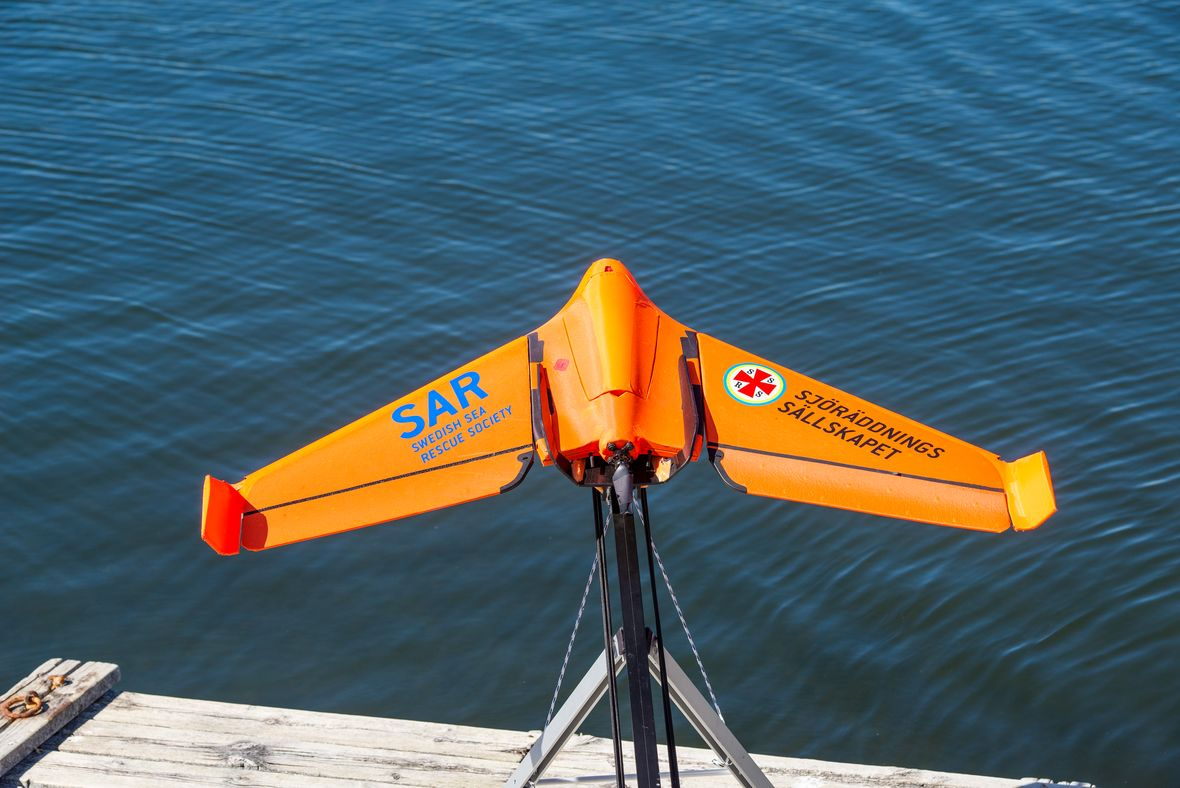
\includegraphics[scale=0.25]{parrot}
    \caption{\ac{uav} platform used for real flight experiments}
    \label{fig:parrot}
\end{figure}


\section{Obstacle avoidance}
To ensure low execution times it is crucial to use an efficient method of checking for collisions between states and $\xobst$. 
In this implementation, the S2Geometry library developed by Google was used \cite{s2geo}. This is a C++ library which contains 
efficient methods to index geometrical objects of any shape, and checking for collisions between different geometries such as points, lines and polygons. 

\section{Wind estimation}
The \ac{ekf} based wind measurement system described in Section \ref{sec:wind_ekf} was used to provide estimates of both $\windspd$ and $\winddir$. A \ac{ma} filter with a 
window size of 2 seconds was used to remove small variations in the measurements.

\section{Landing sequence calculation}
In order to calculate the landing sequence, the optimization problem \eqref{eq:opt_problem_land} is solved. 
This problem was solved with \ac{ipopt} using the \textabbr{CasADi} toolkit, which is a general toolkit for solving nonlinear optimization problems numerically \cite{casadi}.

\section{Motion planner}
The following sections describe implementation details related to the motion planner. 
\subsection{Input set generation}
The input set $\inputs$ was generated using the approach described in Section \ref{sec:motion_prims_wind}. 
It was generated for wind directions $\psi_{w,k}=\{0\degree,20\degree,40\degree,\hdots,340\degree\}$ and desired final course changes
$\Delta\cog=\{20\degree,40\degree,\hdots,180\degree\}$, resulting in a total of 162 inputs for each specific $\windspd$. Symmetries of the system reduce the set of necessary inputs
as solutions for $\Delta\cog=\{-20\degree,-40\degree,\hdots,-180\degree\}$ are simply found by mirroring the $y_E$ coordinate of $u$.
The optimization problem was solved using NOMAD \cite{nomad}, a C++ implementation of the \ac{mads} algorithm.
Cross-track error constraints were defined by $\lambda_d=25$ and $d_{\text{min}}=2.5$ m, \ac{cog} error $\Delta\psi=15\degree$ and wind variation $\delta_W=0.25$. The initial guess for $u$ 
was found by performing a grid search over the values
\begin{equation}
    \actions_{s,\text{init}}=\{(\Delta x_N,\Delta y_E): |\Delta x_N| \leq 300, 0\leq \Delta y_N \leq 300\}
\end{equation}
with a step size of 10 meters and selecting the input with the lowest value of the objective in Equation \eqref{eq:max_opt}.
Simulations of the closed-loop system for the generated inputs $u$, calculated for some different wind directions and $\windspd\in[3.75, 6.25]$ m/s, are shown in Figure \ref{fig:motion_prims}.
\begin{figure}
    \centering
    \subfloat[$\winddir=0\degree$]{
        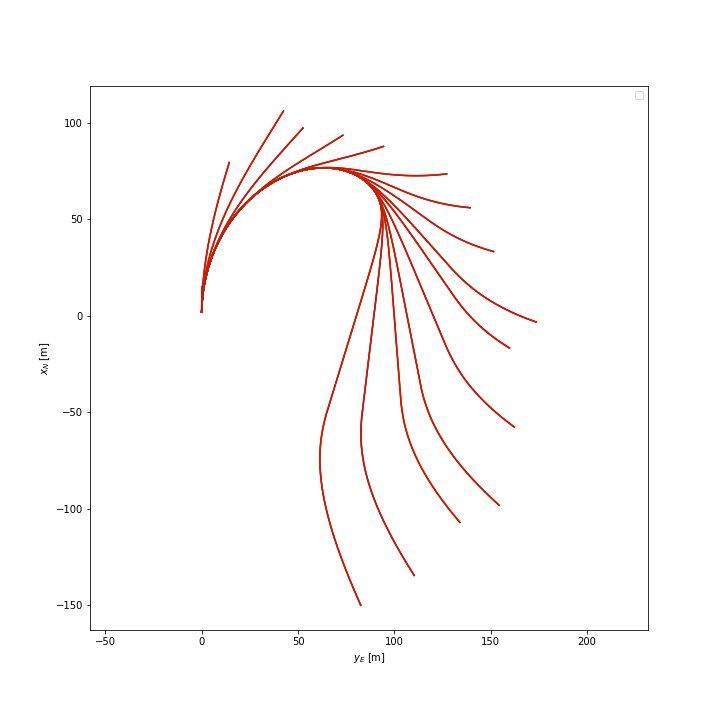
\includegraphics[width=.8\linewidth]{mp_0}
    }\\
    \subfloat[$\winddir=80\degree$]{
        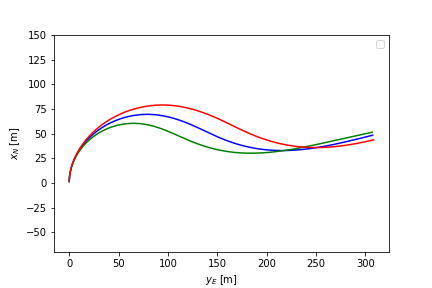
\includegraphics[width=.8\linewidth]{mp_80}
    }
    \caption{Inputs for different wind directions, $\windspd\in[3.75, 6.25]$ m/s}
    \label{fig:motion_prims}
\end{figure}

\subsection{State-space discretization}
To apply graph-search methods, the state-space has to be discretized. In this work the values of $x_N$ and $y_E$ were discretized into cells of size $d=10$ meters, and the 
heading $\psi$ was discretized in steps of $20\degree$. The Hybrid $A^*$ method presented in Section \ref{sec:hybrid-a-star} was used when sampling the state space, allowing continuous values of the state vector $x$ but assigning those to the closest 
discretized state.

\subsection{State expansions}
The step $\text{EXPAND}$ in Algorithm \ref{alg:astar} presented in Section \ref{sec:a-star} has to take both the wind direction $\winddir$ and the heading $\psi$ of $x$ into account. 
Since the inputs in $\inputs$ are generated using initial heading $\psi_0=0$, it is first necessary to calculate the closest relative wind direction
\begin{equation}
    \psi_{w,rel}=\argmin_{\psi_{w,k}\in\{\psi_{w,k}\}}|(\psi-\winddir)-\psi_{w,k}|
\end{equation}
which is used to select the inputs for expansion. When mirroring inputs the wind direction also has to be mirrored, \ie\ 
$\tilde{\psi}_w=360\degree-\winddir$ is used to calculate $\psi_{w,rel}$. The selected inputs also have to be rotated, \ie\ the initial reference $u=(\Delta x_N, \Delta y_E)$ is transformed to 
\begin{equation}
    \tilde{u}=(\cos\psi \Delta x_N + \sin\psi \Delta y_E, -\sin\psi \Delta x_N + \cos\psi \Delta y_E)
\end{equation}
Finally, the expanded states and corresponding costs are found by simulating the closed-loop system \eqref{eq:closed_loop} using each selected $\tilde{u}$ as input. 
The actual wind direction $\winddir$ is used instead of $\psi_{w,k}$ in these simulations.

\subsubsection{Handling perpendicular winds}
A drawback of using straight line-segments as the control reference is that some inputs become problematic when the difference between 
$\psi$ and $\winddir$ is close to $90 \degree$. In this situation, expanding using an input which corresponds to a course change 
 of $\Delta\cog\approx180\degree$ might result in the trajectory controller choosing to fly in tailwind instead of headwind, leading to a large cross track error. This situation is 
 illustrated in Figure \ref{fig:hdg_diff_wind}.

\begin{figure}
    \begin{center}
        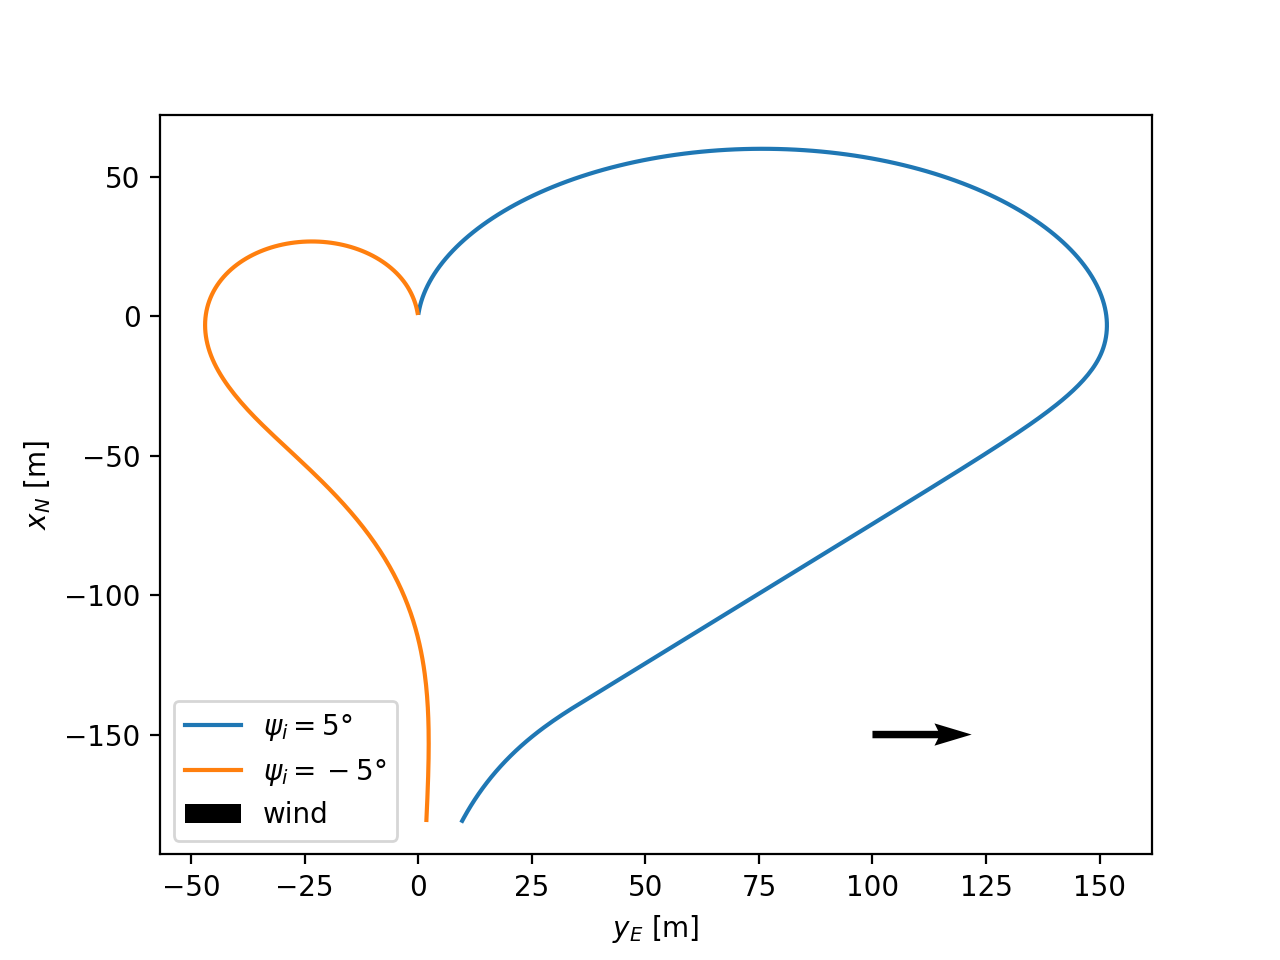
\includegraphics[width=.7\linewidth]{fig/prim_diff_hdg}        
    \end{center}
    \caption{Large cross track error for $\Delta\cog\approx180\degree$ when the wind is perpendicular to \ac{uav} motion}
    \label{fig:hdg_diff_wind}
\end{figure}

This issue was mitigated by defining a set $\psi_{\text{safe}}$ as 
\begin{equation}
    \psi_{\text{safe}}=\{\psi: |\sin\psi|<\frac{1}{\sqrt{2}}\}
\end{equation}
If $|\psi-\winddir|\notin\psi_{\text{safe}}$ during expansion only inputs corresponding to $|\Delta\cog|\leq160\degree$ are used.

\subsection{Heuristic Lookup Table}
The \ac{hlut} was generated using the method in Algorithm \ref{alg:hlut} presented in section \ref{sec:hlut}. The \ac{hlut} was generated using the wind-direction $\winddir=0$, which means that 
entries have to be generated for initial values of $\psi$ from $0\degree$ to $180\degree$ to cover all possibilities. To lookup a query $h(x, x')$ it is then 
necessary to rotate both $x$ and $x'$ by the angle $\winddir$ in order for the query to align with the \ac{hlut}. 

To lower the amount of generated entries the discretization grid was increased to $d=20$ meters when constructing the \ac{hlut}. The set of 
values for which to generate entries was selected as 
\begin{equation}
    \states=\{(x_N,y_E): |x_N|\leq D \cup |y_E| \leq D\}
\end{equation}
for $D=400$ m. To ensure that \ac{hlut} are entries are available for at least states within a smaller set with $D=200$ m, an additional 
$A^*$ search was performed for each such missing state after the initial generation. For $\windspd=5$ m/s the resulting \ac{hlut} consists of 235359 entries.

\section{Waypoint controller}
To send the calculated motion plan and landing sequence to the waypoint controller, these have to be converted to the 
MAVLink protocol which is supported by the ArduPlane autopilot \cite{mavlink}. This interface was implemented using the MAVROS 
plugin in ROS \cite{mavros}. ROS is a modular framework for robotics applications, with API:s available in both Python and C++ \cite{ros}.
